\section{Reimplementing DeepBugs}
\label{sec:replicating_deepbugs}

DeepBugs is structured as shown in Fig. \ref{fig:deepbugs-overview}. DeepBugs first converts a piece of source code (their source code is taken from the 150k JavaScript Dataset \cite{noauthor_150k_nodate}) into an Abstract Syntax Tree (AST). %AST is probably public domain knowledge by now, no worries about citation
The tree is parsed and converted into condensed tokens that represent the relevant code symbols. The symbols are then turned into vectors so that they can be passed into a neural network to classify if the code is buggy or not.

\begin{figure}[h]
    \centering
    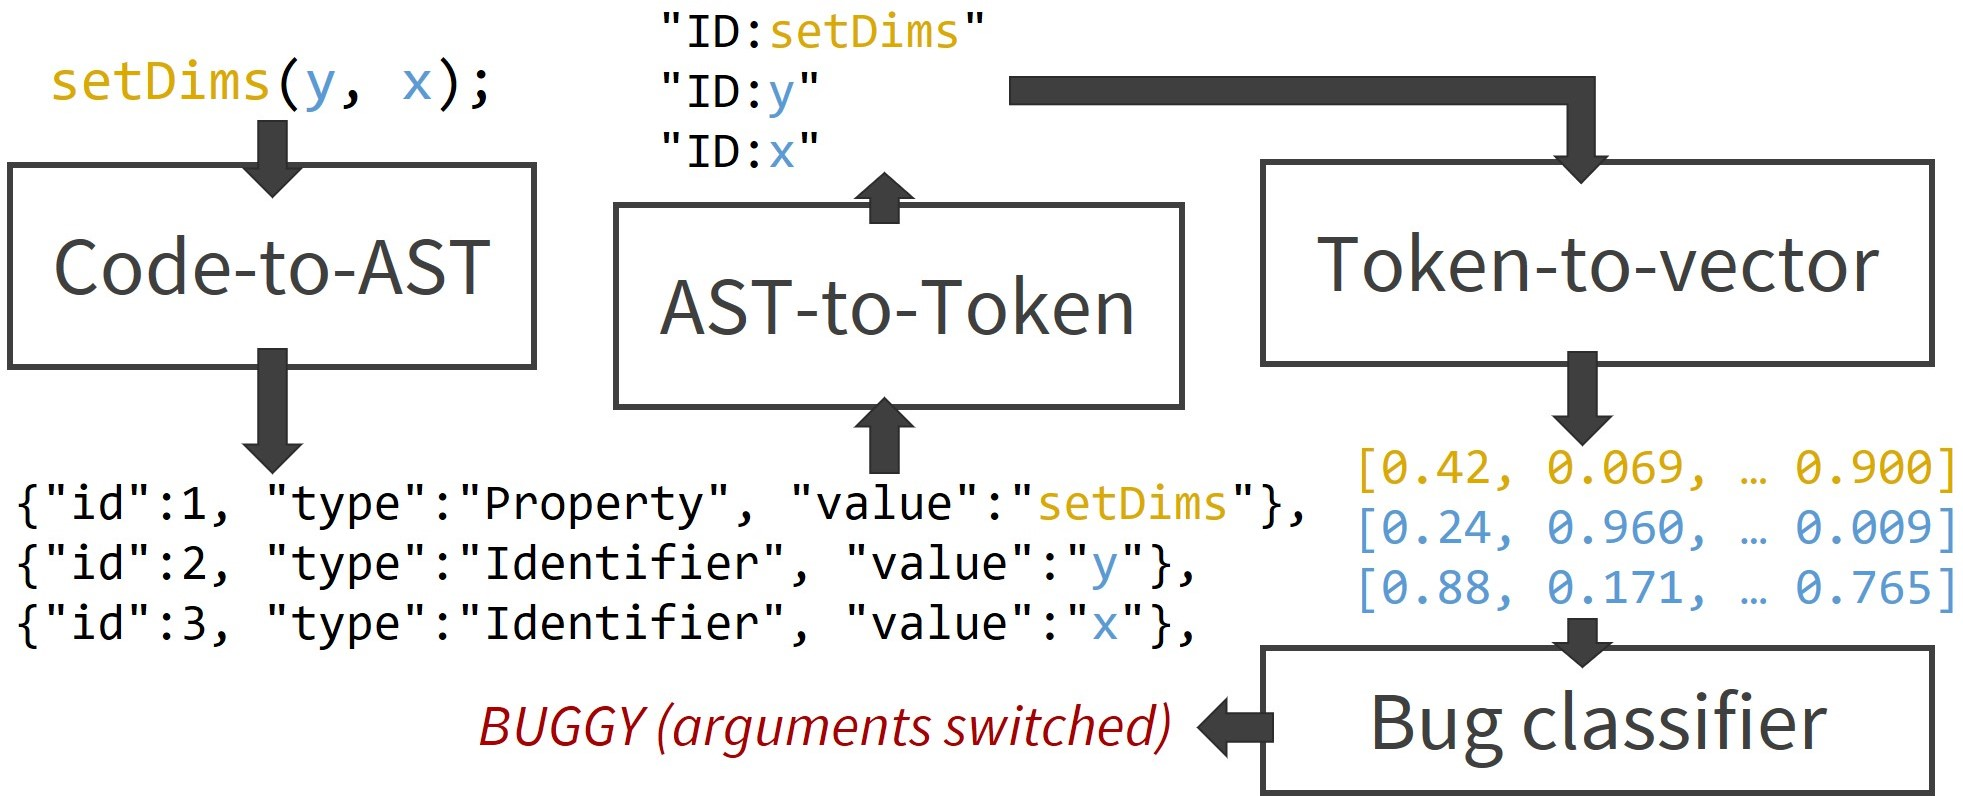
\includegraphics[width=\linewidth]{images/deepbugs-overview.jpg}
    \caption{DeepBugs first converts source code into Abstract Syntax Trees (ASTs) and then into semantic-encoded vectors. The vectors are input to a deep learning model that determines if the source code is buggy. Here, a developer has written a function call for \texttt{setDims(width, height)} using \texttt{setDims(y, x)}. DeepBugs predicts this as ``buggy'' because the system understands that \texttt{x, width} are semantically similar, as are \texttt{y, height}. Thus, it predicts the arguments are swapped; the order should be \texttt{(x, y)}, not \texttt{(y, x)}.}
    \label{fig:deepbugs-overview}
\end{figure}

The DeepBugs framework is designed to detect any name-based bug pattern. Like the original authors, we implement the framework for the ``swapped argument'' bug case. Our reimplementation of DeepBugs is described in the following four steps.

\subsection{Step 1: Code-to-AST}
\label{subsec:step-1}
The original authors used the Acorn JavaScript parser \cite{noauthor_acornjsacorn_2021} to convert JavaScript source code files into a Json formatted Abstract Syntax Tree (AST). For simplicity of testing the swapped-argument bug pattern, we removed AST nodes unrelated to name-base bugs. Our simplified format only uses the \texttt{``children''} AST attribute, which identifies the AST nodes that are acted upon by a given statement or call block. For example, calling some method \texttt{object.methodName(arg1, arg2)} would yield the following simplified AST structure:
\\

\small
\texttt{\{``id'':1, ``type'':``CallExpression'', ``children'':[2,5,6]\},}

\texttt{\{``id'':2, ``type'':``MemberExpression'', ``children'':[3,4]\},}

\texttt{\{``id'':3, ``type'':``Identifier'', ``value'':``object''\},}

\texttt{\{``id'':4, ``type'':``Property'', ``value'':``methodName''\},}

\texttt{\{``id'':5, ``type'':``Identifier'', ``value'':``arg1''\},}

\texttt{\{``id'':6, ``type'':``Identifier'', ``value'':``arg2''\}}\\

\normalsize

This allows us to quickly switch the ordering of the elements in the \texttt{``children''} list and generate swapped-argument bugs.

\subsection{Step 2: AST-to-Token}
\label{subsec:step-2}
For a given bug pattern, not every node in the AST necessarily needs to be evaluated. Further, since each node contains many characters dedicated to represent the node's schema, each relevant group of nodes should be compressed into small tokens that represent the entire group. The tokens can then be vectorized and fed to a neural network for bug classification.

More concretely, for the swapped-argument bug pattern, we are only interested in function names and argument names for any 2-argument function call. To generate tokens, we do the following: For a given AST node, only attempt to generate a token from its \texttt{value} field. If the node does not have a \texttt{``value''} field, derive one from its \texttt{``children''}. The rules we use to generate tokens are similar to those used by the original authors:

\begin{itemize}
    \item A \texttt{CallExpression} with multiple \texttt{Identifier} children can be tokenized separately, with the first child tokenized as the function name, and the remaining children tokenized as the arguments.
    \item A \texttt{MemberExpression} with both an \texttt{Identifier} child and a \texttt{Property} child can be tokenized into the object name and the method/property name, respectively.
    \item Variable names and function names are tokenized as identifiers, with \texttt{``ID:<variable name here>''}.
    \item JavaScript literals of all types are tokenized as 
    \texttt{``LIT:<value>''}.
    \item Other language elements like operands, \texttt{if/else} blocks, \texttt{try/catch} blocks, and \texttt{for} loops are ignored.
\end{itemize}

Using that system, we crawl the entire corpus of code in the 150k JavaScript Dataset, converting each file's AST into a list of tokens. This dramatically compresses the size of our data, distilling only important components. For example, the 6-node AST provided in the Step 1 example (Sec. \ref{subsec:step-1}) would be tokenized into the following list:

\small
\texttt{[``ID:object'', ``ID:methodName'', ``ID:arg1'', ``ID:arg2'']}.
\normalsize

\subsection{Step 3: Token-to-Vector}
\label{subsec:step-3}
To vectorize a token for the neural network bug classifier, the original authors use the Word2Vec \cite{mikolov_efficient_2013} model. Word2Vec can capture lexical similarities between two words, based on the context of the other words surrounding the two words. For example, the letter \texttt{x} and the word \texttt{width} do not necessarily carry similarities on their own. However, in the context of \texttt{setDims()}, they take on similar meanings (i.e., ``width along x-dimension''). Under the CBOW (Collected Bag Of Words) variant, Word2Vec considers a window of words both before and after the word in question to decide the word's vector representation. In our example, this would mean that Word2Vec's output vectors for \texttt{``ID:x''} and \texttt{``ID:width''} would be similar.

To build our Word2Vec model, we first use our AST-to-Token extractor from Step 2 (Sec. \ref{subsec:step-2}) to list all tokens, in order of appearance, for a given JavaScript file's AST. The list of tokens can then be used as a ``paragraph'' of words to feed Word2Vec. We then implement and train our CBOW Word2Vec instance using a window size of 200 tokens (i.e., 100 tokens before the current token, 100 tokens after the current token). To sanity-check our model, we compare the vector similarities of  \texttt{``LIT:true''} with \texttt{``LIT:false''}, \texttt{``LIT:0''}, and \texttt{``LIT:1''} using cosine distance (dot product). We observe that the two true-values are similar to each other (i.e., distance is close to 0), and the two false-values are similar to each other. Meanwhile, the true-values are not similar to the false values (i.e., distance is much farther than 0). This is expected behavior, suggesting that the Word2Vec model is reasonably trained.

\subsection{Step 4: Bug Classifier}
\label{subsec:step-4}
As shown in Fig. \ref{fig:deepbugs-nn}, the DeepBugs bug classifier is a simple neural network that feeds the input through a 20\% dropout regularization layer, a 200-node hidden layer with ReLU activations, another 20\% dropout layer, and a final sigmoidal node to determine the buggy/not buggy prediction. The small size of the network facilitates faster training for different bug patterns.

\begin{figure}[h]
    \centering
    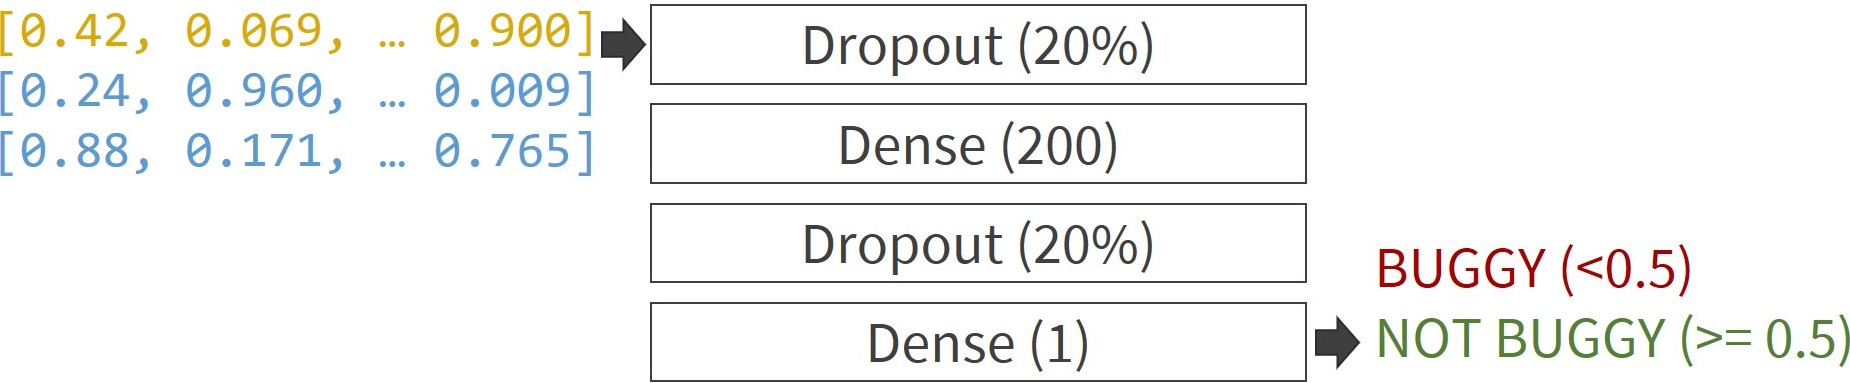
\includegraphics[width=\linewidth]{images/deepbugs-nn.jpg}
    \caption{The Deepbugs classifier is a small neural network that can be rapidly retrained to predict different name-based bugs. As shown, we train our replicated classifier for swapped-argument bug detection.}
    \label{fig:deepbugs-nn}
\end{figure}

Depending on the bug pattern being tested for, the input to the neural network may differ. For the swapped-argument bug, the vectors for the function name and two arguments are concatenated before feeding into the network.



% \section{Experimental Setup}

% \subsection{Problem Statement}
% \label{sec:problem_statement}
% For published research papers, particularly popular ones, it is important for the community to reproduce or replicate the work, thus confirming the validity of the authors' claims.
% Despite being cited repeatedly in the ``Background'' section of other works (DeepBugs has been cited 99 times, according to Google Scholar), DeepBugs has not, to our knowledge, been replicated. Thus, it remains unverified.

% To verify the work detailed by the authors of DeepBugs, we will attempt to replicate their methods. In keeping with the ACM's definitions of ``replication,'' \cite{} if we can implement the algorithms outlined in the DeepBugs paper, run them on the authors' data, and achieve the the authors' 68\% true-positive rate, we will consider our project a success (DeepBugs paper verification is complete).

% If we are unable to achieve the authors' results, we will perform a line-by-line analysis of our implementation. If we cannot find discrepancies between our work and the DeepBugs paper, we will still consider our project a success (DeepBugs paper cannot be verified and should be scrutinized by the community).


% \subsection{Proposed Work}
% \label{sec:proposed_work}
% In this project, we will replicate the DeepBugs paper. As illustrated in Fig. \ref{fig:deepbugs_overview}, the DeepBugs bug detection framework first generates both positive and negative training data from a large dataset of code, then expresses the training data as vectors. A simple binary classifier is then trained; the network's output is either ``TRUE, code is likely bug-free'' or ``FALSE, code likely contains bug.'' Finally, test code can be vectorized and predicted by the neural network. DeepBugs is designed to test for name-based bugs, and the original authors have trained it to identify accidentally swapped arguments and swapped operands.

% \begin{figure}[ht]
%     \centering
%     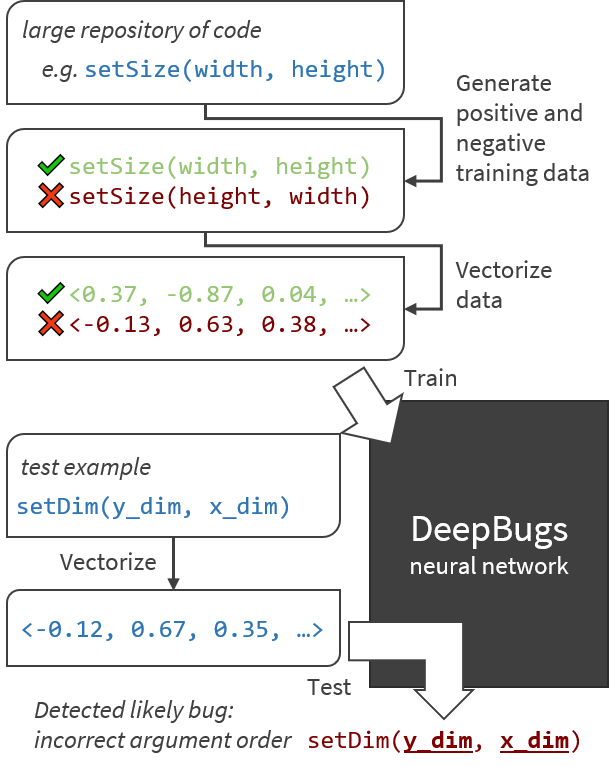
\includegraphics[width=\linewidth]{images/DeepBugs Overview.png}
%     \caption{Overview of the DeepBugs framework.}
%     \label{fig:deepbugs_overview}
% \end{figure}


% \subsection{Generate training data}
% \label{subsec:generate_training_data}
% DeepBugs is trained on large amounts of code. For a given snippet of code, we will create a positive training example (not buggy) and a negative training example (buggy). The original authors supply a large corpus of over 150,000 lines of JavaScript code from which to generate training data; we will use the same corpus. However, we will generate the training examples ourselves.

% We will assume that any given snippet of code from the corpus is likely correct, since the code is pulled from stable commits of well-known open source projects. Therefore, we can use the snippet as a positive example and modify it to become the negative example. As in the original paper, we will first generate an Abstract Syntax Tree (AST) for the code, allowing us to represent the code syntactically as a tree. Then, we can apply a simple AST transformation on the code, e.g. switching the arguments, to create the negative snippets. Both positive and negative examples will be shuffled into the larger dataset.

% \textbf{Verification:} We will verify that our training data generation works correctly by running unit tests. We can then verify the original authors' training examples against our own.

% \subsection{Represent code identifiers as vectors}
% \label{subsec:represent_code_identifiers}
% Because the feedforward classification neural network in DeepBugs requires numerical input, we must translate the training code examples into numerical vectors. This is done through a two-stage process:

% (1) \textit{Vocabulary definition.} Because the DeepBugs classifier must have a fixed input size, the authors set the maximum number of tokens (identifiers and literals) in the code to 10,000 (previously demonstrated to be sufficient in other bug detection experiments). As in the paper, we will select these 10,000 tokens from the code corpus in order of popularity; the remaining tokens will be identified as ``unknown.''

% (2) \textit{Vector encoding by semantic similarity}. In order for DeepBugs to identify accidental coding mistakes, it needs to have an abstract understanding of ``what the developer actually meant to do.'' For example, if trained for swapped arguments on the code snippet \texttt{onComplete(error, result)}, DeepBugs should be able to classify \texttt{onComplete(res, err)} as buggy because \texttt{res} is semantically similar to \texttt{result} - the developer ``actually meant to'' switch the arguments. Therefore, \texttt{res} and \texttt{result} should result in similar vector encodings. This is not necessarily concurrent with lexical similarity - \texttt{rock} and \texttt{rocket} are lexically similar because they share ``rock'' but are not at all semantically similar, so they should have different vector encodings. To achieve this, we will train a Word2Vec network to accomplish semantic encoding for a given code token \cite{mikolov_efficient_2013}.

% \textbf{Verification:} We can check the correctness of our vector representation system with a battery of unit tests that compare the distance between vectors using the standard L2 Norm. We can then verify the original authors' Word2Vec model against our own.

% \subsection{Train and Test DeepBugs neural networks}
% \label{subsec:train_and_test_deepbugs}
% DeepBugs' architecture is illustrated in Fig. \ref{fig:deepbugs_neural_network}. We will implement this classifier and train on our training examples using the same hyperparameters as those found in the paper.

% \begin{figure}[h]
%     \centering
%     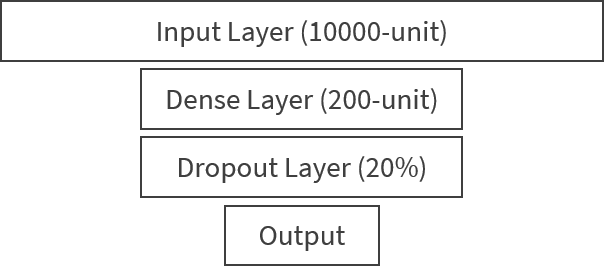
\includegraphics[width=\linewidth]{images/DeepBugs neural network.png}
%     \caption{Architecture of the DeepBugs classifier.}
%     \label{fig:deepbugs_neural_network}
% \end{figure}

% \textbf{Verification:} We will test our implementation using the authors' validation dataset. To further explore DeepBugs' generalization capabilities, we will also create our own test examples with non-JavaScript languages (in particular, other dynamically typed languages like Python and other strictly typed languages like C) and report on our findings.

% \subsection{Dissemination and continued work}
% \label{subsec:dissemination_and_continued}
% Should our project conclude successfully, we may disseminate our replication studies via the ROSE Festival. Additionally, because not every member of our team is well-versed in Python deep learning frameworks like TensorFlow, we estimate the project will take a full semester to complete. However, if we complete the work more quickly, our team plans to perform a replication study of other automated bug detection papers. Monperrus et al.'s \textit{Detecting Missing Method Calls in Object-Oriented Software} \cite{monperrus_detecting_2010} is of particular interest because in contrast to DeepBugs, that work uses hand-crafted statistical methods to find bugs.